\chapter{Representación de ambiente de ejecución}

En este trabajo, se argumenta que las descripciones de los ambientes computacionales es necesaria para la reproducción  del experimento. Además, la información debe ser la suficiente para comparar y detectar las diferencias entre el ambiente original y el reproducido.

Dado que las imágenes Docker son ambientes aislados y independientes, los componentes de software dentro del contenedor si están relacionado al experimento y no existen componentes relacionados a otros experimentos.
Por esta razón, se asegura que las anotaciones no presentarán ruido de otras herramientas o dependencias asociadas.
Para realizar una anotación automática de los paquetes instalados, se propone e implementa un sistema de anotación automático. El sistema requiere el nombre de una imagen existente en un repositorio de DockerHub y opcionalmente los datos del repositorio Git que almacena el archivo Dockerfile. 

Los pasos asociados del sistema anotación:

\begin{enumerate}
	\item Consultar a repositorio de imágenes Docker público o privado los metadatos de la imagen. Anotar los metadatos utilizando la ontología propuesta.
	\item Descargar cada una de las capas asociadas a la imagen Docker.
	\item Sistema anotador consulta a Clair, Clair monta cada una de capas de la imagen, detecta los componentes de software instalados utilizando el sistema de paquete.
	\item Obtener la información de Clair, anotar los datos obtenidos por Clair según la ontología.
	\item Guardar los datos en una base de datos RDF que permita consulta SPARQL.
\end{enumerate} 

%----------------------------------
% 4.1 Semantic models
%----------------------------------
\section{Modelos semánticos}\label{s4.1}
     
En \cite{santana2017reproducibility}, los autores proponen \emph{The Workflow Infrastructure Conservation Using Semantics ontology (WICUS)}. WICUS es ontología OWL2 (Web Ontology Language) que implementa la conceptualización de los principales dominios de la infraestructura computacional. Estos son: Hardware, Software, Workflow y recursos de computo
Los autores definen que los workflows científicos requieren un conjunto de componentes de software, y los investigadores deben conocer cómo desplegar estos componentes para lograr ambiente equivalente.
Considerando que la ontología está relacionada con nuestro trabajo, se utiliza algunas clases y relaciones desde la ontología WICUS:

\begin{description}
	\item [DeploymentPlan:]  Un plan de despliegue está compuesto de todos los pasos. Y el plan de despliegue permite entender al investigador cuáles fueron los pasos requeridos para construir el ambiente computacional.
	\item [DeploymentStep:] Cada paso de despliegue es representado por una línea de comando que realiza la instalación, descarga o configuración del ambiente. La información se obtiene desde el archivo DockerFile
	\item [SoftwareComponent:] Es un componente de software instalado sin una versión específica. 
\end{description} 

Se define el recurso \verb|dockerpedia:SoftwarePackage| como una subclase de \verb|wicus:SoftwareComponent| para definir los componentes instalados por el gestor de paquetes del sistema operativo u otro.
Cada \verb|wicus:SoftwareComponent| tiene una relación \verb|dockerpedia:hasVersion| o \verb|dockerpedia:isVersionOf| que muestra la versión del software instalado.
El recurso \verb|dockerpedia:PackageVersion| puede estar afectado por vulnerabilidades representadas por el recurso \verb|dockerpedia:SoftwareVulnerability|. Y las versiones que reparan la vulnerabilidad se encuentran representadas por \verb|dockerPedia:SecurityRevision|.
Una imagen Docker se representa por \verb|dockerpedia:SoftwareImage| y sus capas por el recurso \verb|dockerpedia:ImageLayer|. Los paquetes instalados en la imagen están relacionado por \verb|vocab:ContainsSoftware| con su imagen.
Finalmente, el sistema operativo es representado por recurso \verb|dockerpedia:OperatingSystem| y cada imagen y capa de la imagen está asociado al recurso.

Una versión completa de la ontología se encuentra disponible en nuestros repositorios \footnote{\url{https://github.com/dockerpedia/ontology/}} y la versión resumida está representada en la figura ~\ref{fig:ontology}. 

\begin{figure}
  \caption{Docker ontology.}
  \centering
    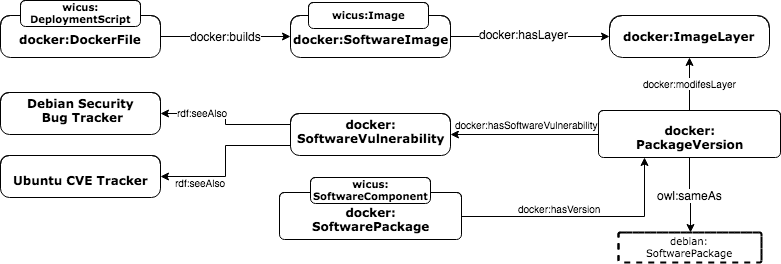
\includegraphics[width=1\textwidth]{Figures/dockerOntologyBasic.png}
    \label{fig:ontology}
\end{figure}

%----------------------
% 4.2 Annotator
%-----------------------
\section{Anotador}\label{s4.2}

El servicio de anotación propuesto cuenta con una interfaz REST para recibir el nombre y la versión de la imagen Docker relacionada con el experimento científico. 
Para almacenar y interactuar con los datos el sistema de anotación utiliza a Apache Jena. Apache Jena es un framework Java gratuito y de código abierto para la construcción de aplicaciones de Web Semántica y Datos Enlazados. El sistema anotador construye los triples relacionado con el experimento, imagen, capas, componentes de software y vulnerabilidades y se envían usando con la API de Apache Jena que serializa los triples utilizando formatos populares como RDF/XML o Turtle.
Esta decisión permite realizar cambios a otra herramienta en caso que Apache Jena no cumpla con los requerimientos de escalabilidad.

El sistema anotación realiza dos tipos de anotaciones: Componentes de software y pasos de construcción.


%--------------------------------------------
% 4.2.1 Building steps annotations
%---------------------------------------------
\subsection{Anotaciones de los pasos de construcción}\label{s4.2.1}

Anotamos el plan de despliegue (Deployment Plan) usando dos métodos. El primero método obtiene los pasos desde el archivo Dockerfile entregado por el usuario, esto permite obtener los pasos y la ubicación de archivo en el repositorio. 
Usando este método se asegura la reconstrucción del ambiente debido a que cualquier archivo necesario por Dockerfile se encuentra en el repositorio Git.
Sin embargo, un usuario puede construir una imagen sin compartir el archivo Dockerfile. En ~\cite{DBLP:conf/semweb/OsorioAV18a} se reporta que el 30\% de las imágenes Docker en DockerHub enlanza su archivo Dockerfile. 
Por lo tanto, sino existe información del Dockerfile el sistema anotación utiliza el manifesto de la imagen Docker. Según \footnote{\url{https://docs.docker.com/registry/spec/manifest-v2-2/}} para conocer los pasos, el manifiesto de la imagen provee la configuración y el conjunto de las capas de la imagen

Algunos atributos importantes son:

\begin{description}
	\item [name:] \textit{string} nombre de la imagen
	\item [tag:] \textit{tag} version de la imagen
	\item [architecture:] \textit{string} arquitectura del servidor en cuál la imagen ha sido construido. Esta información actualmente no es utilizada por Docker.
	\item [fsLayers:] \textit{array} lista de las capas que componente la imagen.
		La estructura contiene los siguiente campos:
		\begin{description}
			\item [blobSum:] es un identificador utilizando una función de hash sha256 para cada capa de la imagen 
		\end{description}
	\item [history]: \textit{array} Es una lista de datos históricos no estructurados para la compatibilidad con la v1. Contiene el ID de la capa de imagen y el ID de las capas principales de la capa. El historial es una estructura que consta de los siguientes campos:
	\begin{description}
		\item[v1Compatibility]:  \textit{string} V1Compatibilidad es la información de compatibilidad de V1 en bruto. Esto contiene el objeto JSON que describe la V1 de esta imagen. Una V1Compatibilidad es una estructura que consta de los siguientes campos:
		
		\begin{description}
			\item [Id:] \textit{string} ID de la capa utilizando hash sha256			\item [Parent:] \textit{string} ID de la capa madre utilizando hash sha256
				\item [ContainerConfig:] \textit{string} El comando que construyó la capa
		\end{description}
	\end{description}
\end{description}



%--------------------------------------------
% 4.2.2 Software Components annotations
%---------------------------------------------
\subsection{Anotaciones de componentes de software}\label{s4.2.2}

Para lograr la anotación de los componentes de software se utiliza los gestores de paquetes del sistema, un gestor de paquete es una colección de herramientas de software que automatizan la instalación, actualización, configuración y eliminación de componentes de software. 
Los gestores que paquetes se clasifican en dos tipos: gestor de paquetes del tipo sistema y general:

\begin{description}
	\item  [Gestor de paquetes de sistema:] son aquellos vinculados al sistema operativo (e.g., apt de familia Debian, yum de familia RedHat).
	\item [Gestor de paquetes generales:] son aquellos externos que normalmente son utilizados para instalar un componentes de software de tercero ó un lenguaje especifico (e.g., pip, conda, npm). Conda es un sistema paquete frecuentemente utilizado por investigadores al estar relacionado con Jupyter Notebook.
\end{description}

%--------------------------------------------
% 4.2.2 Desafíos del sistema de anotación
%---------------------------------------------
\subsection{Desafíos del sistema de anotación}\label{s4.2.3}

La descripción de los componentes de software es fundamental para realizar cuantificar la similitud entre dos o más ambientes computacionales.
Un enfoque común para detectar los componentes de software guardar o detectar los comandos que realizan la instalación de software. Por ejemplo, la figura \ref{lst:tensorflow} muestra los comandos para instalar los componentes de la imagen TensorFlow. 

\begin{lstlisting}[caption={Ejemplo de instalación de dependencias para la imagen TensorFlow},label={lst:tensorflow},language=bash]
apt-get install -y --no-install-recommends \
        build-essential \
        curl \
        libfreetype6-dev \
        libhdf5-serial-dev \
        libpng12-dev \
        libzmq3-dev \
        pkg-config \
        python \
        python-dev \
        rsync \
        software-properties-common \
        unzip	
\end{lstlisting}

El enfoque detectaría los componentes: build-essential, curl, libfreetype6-dev, libhdf5-serial-dev, libpng12-dev, libzmq3-dev, pkg-config, python, python-dev, rsync, software-properties-common y unzip. Sin embargo, este enfoque no obtiene información sobre las versiones o las dependencias del software. Utilizando el  enfoque propuesto, se puede terminar que el línea anterior instala 184 paquetes.

Como prueba de generación y considerando la popularidad de Jupyter Notebook y conda en la comunidad científica, se extiende Clair para detectar los paquetes instalados por Conda en la imagen. La propuesta incluye e implementa la extensión de Clair para detectar los componentes de software instalados por Conda

En la figura se muestra algunos de los paquetes instalado en la imagen de un workflow construido con Pegasus \ref{lst:packages-pegasus}, en la figura \ref{lst:vulnerability} se muestra una vulnerabilidad de paquete glibc instalado en la imagen Pegasus.
\begin{lstlisting}[caption={Ejemplo de triples que muestran los componentes de software de la imagen Pegasus},label={lst:packages-pegasus},language=bash]

<http://dockerpedia.inf.utfsm.cl/resource/SoftwareImage/dockerpedia-pegasus_workflow_images%3Apegasus-4.8.5>
        vocab:containsSoftware  <http://dockerpedia.inf.utfsm.cl/resource/PackageVersion/libxcb-1.11.1-1ubuntu1>, <http://dockerpedia.inf.utfsm.cl/resource/PackageVersion/cryptsetup-2%3A1.6.6-5ubuntu2.1> , <http://dockerpedia.inf.utfsm.cl/resource/PackageVersion/e2fsprogs-1.42.13-1ubuntu1> , <http://dockerpedia.inf.utfsm.cl/resource/PackageVersion/dbus-glib-0.106-1> , <http://dockerpedia.inf.utfsm.cl/resource/PackageVersion/libxmu-2%3A1.1.2-2>
\end{lstlisting}

\begin{lstlisting}[caption={Ejemplo de triples de la vulnerabilidad de glibc},label={lst:vulnerability},language=bash]
<http://dockerpedia.inf.utfsm.cl/resource/SoftwareVulnerability/CVE-2018-6485>
vocab:affectOS     <http://dockerpedia.inf.utfsm.cl/resource/OperatingSystem/ubuntu%3A16.04> , <http://dockerpedia.inf.utfsm.cl/resource/OperatingSystem/debian%3A9> ;
vocab:description  "An integer overflow in the implementation of the posix_memalign in memalign functions in the GNU C Library (aka glibc or libc6) 2.26 and earlier could cause these functions to return a pointer to a heap area that is too small, potentially leading to heap corruption." ;
vocab:link         "https://security-tracker.debian.org/tracker/CVE-2018-6485" , "http://people.ubuntu.com/~ubuntu-security/cve/CVE-2018-6485" ;
vocab:severity     "High" .
\end{lstlisting}
